%%
%%  Department of Electrical, Electronic and Computer Engineering.
%%  EPR400/2 Final Report - Section 3.
%%  Copyright (C) 2011-2021 University of Pretoria.
%%

\section{Design and implementation}

\subsection{Things I made}
\begin{itemize}
    \item Laser turret housing.
    \item Worked out the speed, torque, and step size required for the stepper motors.
    \item Interfaced with stepper motors using GPIO pins to drive the stepper motor drivers.
    \item Mapping between camera pixels and real-world co-ordinates. Had to do camera calibration and account for different perspectives of camera and turret.
    \item Calculate steps from angle required based on distance using Pythagoras.
    \item Distinguish between laser reflections using the geometry of the laser turret.
    \item Laser detection from first principles optimised with GPU kernels. 1. Gaussian smoothing, 2. Binarise with threshold, 3. Morphological operations (closing and opening), 4. Connected components labelling, 5. Find centroids of connected components, 6. Distinguish laser detections with turret geometry.
    \item Mosquito detection. Same image processing steps expect step 2 is either a less than threshold or background subtraction.
    \item Mosquito tracking using SORT algorithm. (Kalman filter and Hungarian algorithm).
    \item Laser turret PID controller. Must still be tuned because the error calculated is inaccurate. Should tuning be done without developing a model? Or should a model be developed? How do you develop a model?
    \item Feedback for turret. The current steps are saved at the instance that the frame is captured. The frame is then processed using the laser detection system. The pixel co-ordinates are converted to steps. The step error is calculated and added to the current steps.
    \item System integration on embedded system running in real-time on multiple threads.
\end{itemize}


\subsection{Design summary}

This section summarises the project design tasks and how they were
implemented (see \autoref{tab:design_summary}).

\begin{table}[H]
    \centering
    \begin{tabularx}{\textwidth}{|X|X|X|}
        \hline
        \textbf{Deliverable or task}                                                           & \textbf{Implementation} &
        \textbf{Completion of deliverable or task, and section in the report}
        \\
        \hline
        The mosquito detection subsystem had to be designed and implemented by the student.    &
        The mosquito detection subsystem was designed and implemented from first principles.   &
        Completed.
        \\
        \hline
        The laser detection subsystem had to be designed and implemented by the student.       &
        The laser detection subsystem was designed and implemented from first principles.      &
        Completed.
        \\
        \hline
        The laser turret control subsystem had to be designed and implemented by the student.  &
        The laser turret control subsystem was designed and implemented from first principles. &
        Completed.
        \\
        \hline
        The mosquito tracking subsystem had to be designed and implemented by the student.     &
        The mosquito tracking subsystem was designed and implemented from first principles.    &
        Completed.
        \\
        \hline
        The various subsystems had to be integrated on a real-time embedded system.            &
        The various subsystems were integrated on a real-time embedded system.                 &
        Completed.
        \\
        \hline
        Appropriate motors needed to be selected for the laser turret.                         &
        The stepper motors were selected based on the requirements of the laser turret.        &
        Completed.
        \\
        \hline
    \end{tabularx}
    \caption{Design summary.}
    \label{tab:design_summary}
\end{table}


\subsection{Theoretical analysis and modelling}

\subsubsection{Mapping pixel co-ordinates to metric co-ordinates}
% \sout{To control the laser turret the setpoint and laser position detected with the camera must be converted from the pixels in the camera's co-ordinate frame to the turret's co-ordinate frame. This is done using the camera's intrinsic and extrinsic parameters. The camera's intrinsic parameters are used to convert the pixels to a ray in the camera's co-ordinate frame. The camera's extrinsic parameters are used to convert the ray in the camera's co-ordinate frame to a ray in the turret's co-ordinate frame. The ray in the turret's co-ordinate frame is then converted to the turret's setpoint and laser position. The intrinsic and extrinsic parameters are found using camera calibration.}

To control the laser, its position must be known in the world co-ordinate frame. The laser position was measured using a camera, thus the camera's pixel co-ordinate frame must be mapped to the world co-ordinate frame. To perform this mapping a camera model is required. The forward imaging model of a camera is shown in \autoref{fig:camera_forward_imaging_model}.
\begin{figure}
    \centering
    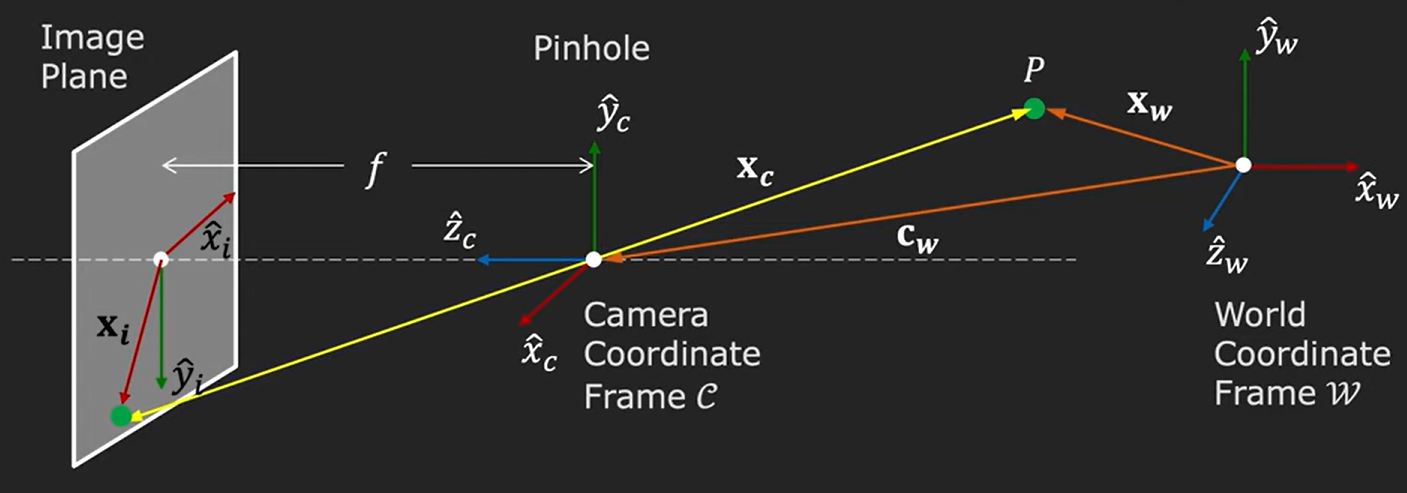
\includegraphics[width=0.8\textwidth]{figures/camera/forward_imaging_model.png}
    \caption{Forward imaging model of a camera. CITE}
    \label{fig:camera_forward_imaging_model}
\end{figure}

Using the forward imaging model the pixel distance was mapped to the metric distance for the x-axis with
\begin{equation}
    X = Z \times \left( \frac{x - x_{ref}}{f_x} \right)
    \label{eq:pixel_to_metric}
\end{equation}

where $Z$ is the depth camera with respect to the world co-ordinate frame, $x$ is the pixel of interest, $x_{ref}$ is the reference pixel, and $f_x$ is the effective focal length of the camera. Similarly, the pixel distance was mapped to the metric distance for the y-axis.

The effective focal length of the camera $f_x$ was determined through camera calibration.

\subsubsection{Camera calibration}
\paragraph{Intrinsic parameters}\mbox{}\\
These parameters are inherent to the camera and remain constant unless the camera's internal settings (like focus) are changed. They are typically found by calibrating the camera using multiple views of a known pattern (like a checkerboard).

\begin{itemize}
    \item \textbf{Camera Matrix (K)}: Defines the camera's internal characteristics. The principal components are:
          \begin{equation}
              K = \begin{bmatrix}
                  f_x & 0   & c_x \\
                  0   & f_y & c_y \\
                  0   & 0   & 1   \\
              \end{bmatrix}
          \end{equation}\\
          where \(f_x\) and \(f_y\) are the focal lengths in pixels and \(c_x, c_y\) are the co-ordinates of the principal point. The principal point is the pixel co-ordinate where the camera's principal axis intersects the image plane.

    \item \textbf{Distortion Coefficients (D)}: Captures lens distortion. This is a vector with up to 5 elements in the common "plumb-bob" model of OpenCV
          \[
              D = [k_1, k_2, p_1, p_2, k_3]
          \]
          where \(k_1, k_2, k_3\) are radial distortion coefficients and \(p_1, p_2\) are tangential distortion coefficients.
\end{itemize}

\paragraph{Extrinsic Parameters}\mbox{}\\
These parameters capture the camera's orientation and position concerning the world or an external reference frame.

\begin{itemize}
    \item \textbf{Rotation Vector (rvec)}: Represents the orientation of the camera. It's a 3x1 vector used to derive the rotation matrix \( R \).

    \item \textbf{Translation Vector (tvec)}: Represents the position of the camera. It's a 3x1 vector capturing the translation in X, Y, and Z directions.
\end{itemize}

They represent the position and orientation of the camera relative to the world (or in your case, the turret's frame). Every time you move the camera or change the scene, these parameters would change. These are found using functions like \verb|solvePnP| in OpenCV, which computes the pose of an object given some known 3D points on the object and their corresponding 2D projections in the image.

\subsubsection{SORT tracking}

\subsection{Simulation and Prototyping}
Detection and tracking done in python with videos.


\subsection{Hardware design}
\textit{Turret inspired by 2d laser scanners. Motor step resolution, speed, and torque calculations. Motor driver selection based on microstepping capabilities. Turret CAD design. Math translation between angle and distance of laser.}

\subsubsection{Mosquito enclosure and system positioning}
\newcommand{\enclosureWidthCM}{90} % cm
\newcommand{\enclosureHeightCM}{38} % cm
\newcommand{\enclosureDepthCM}{32} % cm

The mosquitoes were placed inside an enclosure with a white lining and a glass front panel for the laser beam to shine through. The enclosure is a rectangular prism with dimensions $\enclosureWidthCM \times \enclosureHeightCM \times \enclosureDepthCM$ cm as seen in \autoref{fig:mosquito_enclosure_dimensions}. Internal lighting was added to the enclosure to ensure contrast between the background and the mosquitoes and to minimise the camera noise. The laser turret and the camera were placed outside the enclosure in known positions relative to the enclosure. The bracket, shown in \autoref{fig:system_positioning_bracket}, was designed to hold the laser turret and the camera in place relative to the mosquito enclosure.

\begin{figure}[h]
    \centering
    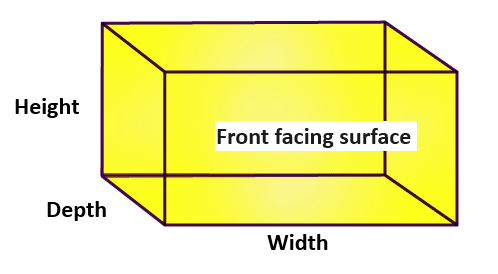
\includegraphics[width=0.5\textwidth]{figures/hardware_design/rectangular_prism.png}
    \caption{Mosquito enclosure dimensions.}
    \label{fig:mosquito_enclosure_dimensions}
\end{figure}

\begin{figure}[h]
    \centering
    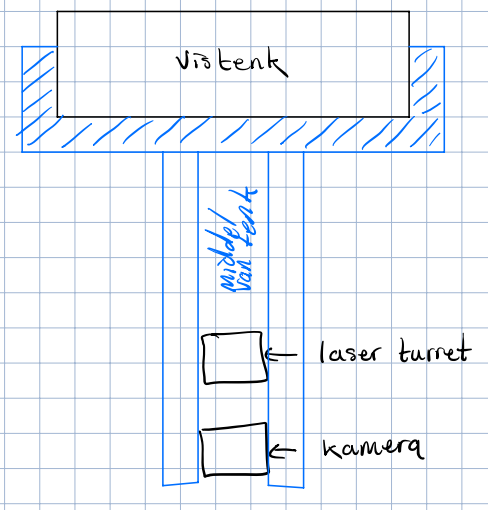
\includegraphics[width=0.5\textwidth]{figures/hardware_design/positioning_bracket.png}
    \caption{System positioning bracket.}
    \label{fig:system_positioning_bracket}
\end{figure}

\subsubsection{Laser turret design}

The laser turret design was inspired by commercial two-axis laser scanners. A schematic for a typical two-axis laser scanner can be seen in \autoref{fig:two-axis-scanner-schematic}. The mirrors \hl{are} connected directly to the output shaft of the motor. The origin of the laser turret \hl{is} where the laser beam shines orthogonal to the mosquito plane, which occurs when the two mirrors \hl{are} at 45$\degree$ relative to the angle of the laser beam when the origin of the laser beam is parallel to the mosquito plane. When a single axis of the laser turret is considered it can be seen that a right triangle is formed between the laser turret and the mosquito plane as shown in \autoref{fig:mirror_angle}. Using the properties of a right triangle the mirror angle $\theta$ required to shine the laser a distance $\pm x$ from the origin of the laser turret can be calculated using
\begin{equation}
    \theta = \arctan{\left(\frac{\pm x}{z}\right)}
    \label{eq:mirror_angle}
\end{equation}
where $z$ is the distance between the turret and the mosquito plane.

\begin{figure}[h]
    \centering
    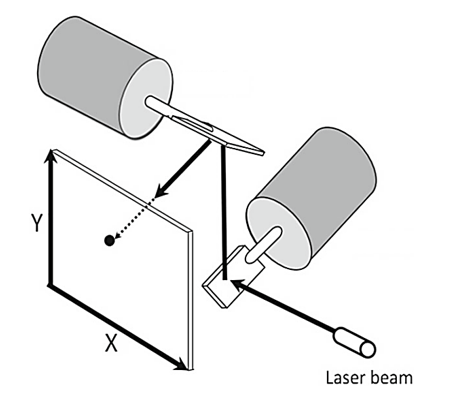
\includegraphics[width=0.5\textwidth]{figures/hardware_design/two_axis_scanner.png}
    \caption{Two-axis laser scanner schematic. This figure was modified from \cite{two-axis-scanner-schematic}.}
    \label{fig:two-axis-scanner-schematic}
\end{figure}

\begin{figure}[h]
    \centering
    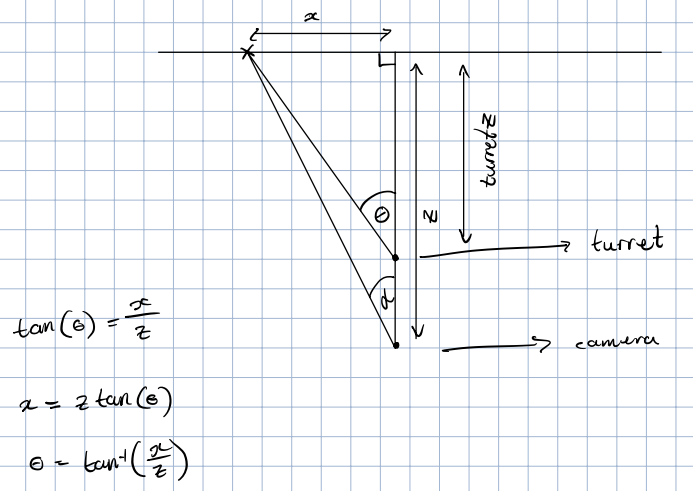
\includegraphics[width=0.5\textwidth]{figures/hardware_design/mirror_angle.png}
    \caption{Mirror angle calculation.}
    \label{fig:mirror_angle}
\end{figure}

The specific geometry of the laser turret was designed with the goal to practically obtain a sufficiently small lateral step size of the laser on the mosquito plane, while maintaining sufficient speed.

\paragraph{Lateral step size and speed}\mbox{}\\
\newcommand{\requiredLatStepSizeMM}{2} % mm
The lateral step size of the laser must be on the order of $\requiredLatStepSizeMM$ mm (size of mosquito plus size of laser).

\newcommand{\requiredLatSpeedMPS}{1} % m/s
The required lateral speed is determined in accordance with the field specifications the longest length of the mosquito enclosure \hl{is} \hl{1~m}. To ensure that the laser could illuminate the set point within \hl{2} seconds of receiving a step input it was assumed that the laser must be able to move with a velocity $v$ of least \requiredLatSpeedMPS~m/s opposed to 0.5~m/s required to move the 1~m length of the mosquito enclosure within 2 seconds. This was done to accommodate for the settling time of the control system. This is also faster than the top speed of a mosquito which is 0.67~m/s according to SOURCE.

\paragraph{Lateral to angular step size}\mbox{}\\
\label{par:lateral_to_angular_step_size}
In the design of the laser turret there were multiple dimensions that were dependent on each other, it is up to the designer to choose certain practical dimensions from which the rest of the dimensions can be calculated. In this design the dimensions of the mirrors were chosen for practicality as $30 \times 15$ mm. These dimensions will be used throughout the rest of the design.

The turret axis on which the laser beam is first incident on will be referred to as the first axis and the other axis will be referred to as the second axis for the remainder of this discussion. The rotation range of the first axis is bounded by the geometry of the turret since the laser beam reflected from the first axis must be incident on the second axis. With the chosen mirror dimensions, the maximum angle through which the first axis can rotate from the origin (45$\degree$ point) is $\theta_{max} =\pm 20\degree$ (add conservatively estimated) resulting in a $40\degree$ range of motion. This was determined geometrically in \autoref{fig:turret_motion_range}. The lines representing the mirrors in \autoref{fig:turret_motion_range} are 30~mm long and the whole figure is drawn to scale. The rotation range of the second axis is not bounded by the geometry of the turret since the laser beam reflected from the second axis is incident on the mosquito plane. Therefore, the turret was oriented such that the first axis moves the laser beam parallel to the shorter width of the mosquito enclosure and the second axis moves the laser beam parallel to the longer length of the mosquito enclosure.

To maximise the angle through which the turret must rotate to move the laser beam across the height of the mosquito enclosure the minimum distance $z_{min}$ between the turret and the mosquito plane was determined by rearranging \autoref{eq:mirror_angle} to give
\begin{equation}
    z = \frac{\pm x}{\tan{\theta}}.
    \label{eq:distance_calculation}
\end{equation}
where $x = \enclosureHeightCM$~cm is the height of the mosquito enclosure. The minimum distance $z_{min}$ was calculated by substituting $\theta_max = 20\degree$ into \autoref{eq:distance_calculation} to give

\FPeval{\zMinCM}{round(\enclosureHeightCM/tan(20*pi/180), 1)}
\begin{equation}
    z_{min} = \frac{\enclosureHeightCM \text{cm}}{\tan{20\degree}} = \zMinCM. \text{cm}.
    \label{eq:z_min_calculation}
\end{equation}

The required motor step resolution was calculated by substituting $x_{min}$ and $z_{min}$ into \autoref{eq:mirror_angle} to give
\pgfmathsetmacro{\stepRes}{atan2(\requiredLatStepSizeMM, \zMinCM*10)}
\begin{equation}
    \arctan\left({\frac{x_{min}}{z_{min}}}\right) = \arctan\left({\frac{\requiredLatStepSizeMM \text{mm}}{\zMinCM \text{cm}}}\right) = \stepRes\degree
    \label{eq:step_resolution_calculation}
\end{equation}

\begin{figure}[h]
    \centering
    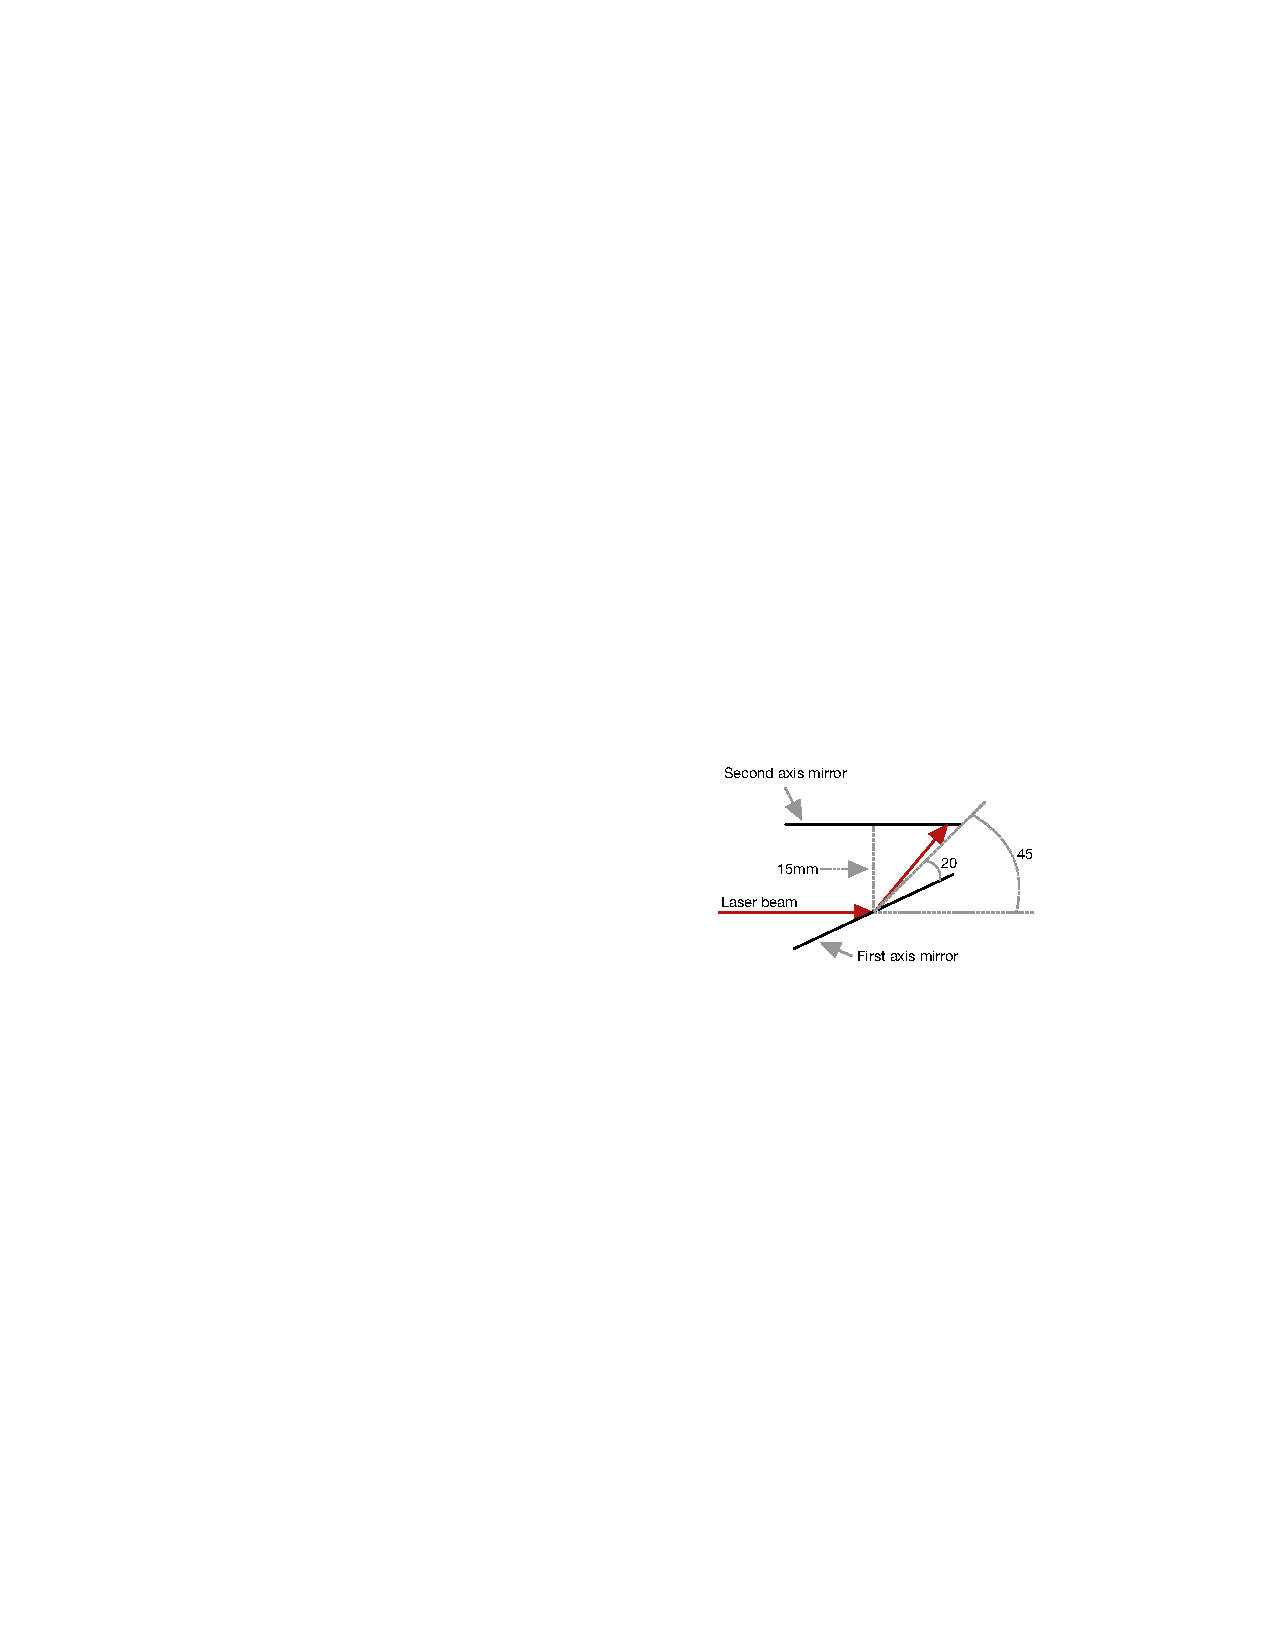
\includegraphics[width=0.6\textwidth]{figures/hardware_design/rotation_range_of_first_axis.pdf}
    \caption{Rotation range of first axis with chosen mirror dimensions.}
    \label{fig:turret_motion_range}
\end{figure}

\paragraph{Lateral speed to angular speed}\mbox{}\\
From \autoref{par:lateral_to_angular_step_size} it is known that
\pgfmathsetmacro{\enclosureHeightM}{\enclosureHeightCM/100}\enclosureHeightM
\begin{equation}
    \begin{aligned}
                 & \SI{\enclosureHeightM}{\meter\per\second} = \SI{40}{\degree\per\second}                                                            \\
        \implies & \enclosureHeightM \times \frac{\requiredLatSpeedMPS}{\enclosureHeightM} = 40 \times \frac{\requiredLatSpeedMPS}{\enclosureHeightM} \\
        \implies & \SI{\requiredLatSpeedMPS}{\meter\per\second} = \pgfmathsetmacro{\result}{40/\enclosureHeightM} \SI{\result}{\per\second}
    \end{aligned}
\end{equation}
The angular speed required to move the laser beam at a lateral speed $v = \SI{\requiredLatSpeedMPS}{\meter\per\second}$ was calculated with $\theta_{max}$ determined in \autoref{par:lateral_to_angular_step_size} using
\begin{equation}
    \omega = v \times \theta_{max}.
    \label{eq:angular_velocity_calculation}
\end{equation}

% Thus, the required angular velocity $\omega_f$ is given by (if assumed that the first axis will cover the width, thus it must actually be faster)
% \begin{equation}
%   \omega_f = v \times \theta = 1 \text{m/s} \times 40\degree \times \frac{\pi}{180} = 0.698 \text{rad/s}.
%   \label{eq:angular_velocity_calculation}
% \end{equation}





\subsubsection{Motor requirements}
\sout{The motor requirements were determined based on system requirement 4 (The laser must be able to illuminate the set point within 2 seconds accurate to within 1~mm.).}

The need for precise position control of the laser meant that only stepper and servo motors were considered. The required torque and required \gls{rpm} was calculated to enable appropriate motor selection. \sout{and the resulting laser step size on the mosquito plane were calculated.} In the calculations only a single axis of the turret was considered since the motors and mirrors for both axes \hl{will be} identical and operate independently.

\begin{figure}
    \centering
    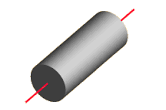
\includegraphics[scale=1]{figures/hardware_design/cylinder_central_axis.png}
    \caption{Central axis of a cylinder.}
    \label{fig:cylinder_central_axis}
\end{figure}

The required torque $\tau$ was calculated using
\begin{equation}
    \tau = I\alpha
    \label{eq:torque}
\end{equation}
where $I$ is the moment of inertia and $\alpha$ is the angular acceleration.

The moment of inertia for the mirror was calculated by \hl{assuming} the mirror was solid cylinder with diameter $d$ equal to the width of the mirror. This will produce an inflated moment of inertia, however, this is not a concern since having extra torque is not a problem. The moment of inertia $I$ of a cylinder with rotation about its central axis as seen in \autoref{fig:cylinder_central_axis} is given by
\begin{equation}
    I = \frac{1}{2}Mr^2
    \label{eq:moment_of_inertia}
\end{equation}
where $M$ is the mass of the cylinder and $r = \sfrac{d}{2}$ is the radius of the cylinder. The mass of the cylinder $M$ was calculated using the density of glass $\rho = 2500 \text{kg/m}^3$ and the volume of the cylinder $V$ given by
\begin{equation}
    V = \pi r^2 h.
    \label{eq:cylinder_volume}
\end{equation}
The height $h$ and radius $r$ of the cylinder was determined by assuming practical dimensions for the mirror. The dimensions of the mirror was assumed to be 30~mm by 15~mm. Thus, the mass of the mirror $M$ is given by
\begin{equation}
    M = \rho V = 2500 \text{kg/m}^3 \times \pi \left(\frac{0.015}{2} \text{m}\right)^2 0.03 \text{m} = 0.01325 \text{kg} = 13.25 \text{g}.
    \label{eq:cylinder_mass}
\end{equation}
Given the above assumptions, the moment of inertia $I$ was calculated as
\begin{equation}
    I = \frac{1}{2}Mr^2 = \frac{1}{2} \times 0.01325 \text{kg} \times \left(\frac{0.015}{2} \text{m}\right)^2 = 1.172 \times 10^{-7} \text{kg} \cdot \text{m}^2.
    \label{eq:cylinder_moment_of_inertia}
\end{equation}

The angular acceleration of the motor $\alpha$ is calculated by
\begin{equation}
    \alpha = \frac{\Delta\omega}{\Delta t}
    \label{eq:angular_acceleration}
\end{equation}
where $\Delta\omega = \omega_f - \omega_i$ is the change in angular velocity and $\Delta t$ is the change in time.  This velocity was translated into the angular velocity $\omega_f$ using
\begin{equation}
    \omega = v \times \theta_{max}
    \label{eq:angular_velocity}
\end{equation}
where $\theta_{max}$ is the angle through which the mirror must rotate to produce a 1~m lateral displacement of the laser on the mosquito plane.

The change in time $\Delta t$ was determined by assuming the laser must be able to accelerate from a stand still to 1~m/s extremely rapidly to ensure that the motors could respond to the irregular flight pattern associated with a mosquito. It was assumed that this acceleration must occur within 10~ms.

Thus, the required angular acceleration $\alpha$ is given by
\begin{equation}
    \alpha = \frac{\Delta\omega}{\Delta t} = \frac{0.698 \text{rad/s}}{0.01 \text{s}} = 69.8 \text{rad/s}^2.
    \label{eq:angular_acceleration_calculation}
\end{equation}
and thus the required torque $\tau$ is given by
\begin{equation}
    \tau = I\alpha = 1.172 \times 10^{-7} \text{kg} \cdot \text{m}^2 \times 69.8 \text{rad/s}^2 = 8.17 \times 10^{-6} \text{N} \cdot \text{m}.
    \label{eq:torque_calculation}
\end{equation}


\subsection{Hardware implementation}
\gls{gpio} interfacing with stepper motor driver.


\subsection{Software design}
\textit{Mapping between pixels and real distance. Mosquito detection and tracking. Laser detection and tracking. \gls{pid} controller. Feedback for turret. Distinguishing between laser reflections.}

\subsubsection{Mosquito and laser detection}
It was assumed that the mosquitoes would be the only dark blobs in the enclosure and that the laser and its reflections would be the only bright blobs in the enclosure. The video frame would be cropped such that only the back wall of the enclosure is visible.

The detection system was designed to work with a red laser because the computational complexity could then be decreased by only considering the red channel of the \gls{rgb} frame.

The mosquito detection was designed to detect dark blobs in the enclosure and would not be able to distinguish between mosquitoes and other dark blobs. The laser detection was designed to detect bright blobs in the enclosure and would not be able to distinguish between the laser and its reflections. The mosquito and laser detection processes are similar in nature. The basic detection process flow is shown in \autoref{fig:detection_process_flow}.

\begin{figure}[h]
    \centering
    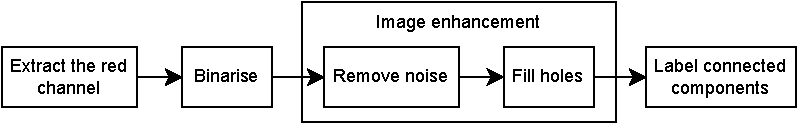
\includegraphics[width=0.8\textwidth]{figures/detection/detection_process_flow.pdf}
    \caption{Detection process flow.}
    \label{fig:detection_process_flow}
\end{figure}

The only difference between the mosquito and laser detection is the binarisation step.

\paragraph{Binarisation}\mbox{}\\
Thresholding or bg sub.

\paragraph{Morphological operations}\mbox{}\\
The respective binarised frames are subject to noise, holes, and erroneously joint or disjointed sections. This can be resolved using morphological operations. Morphological operations work by passing a structuring element over the pixels in a image and performing a logical operation on the pixels in the image that are covered by the structuring element.

The noise and erroneously joint sections are removed using the morphological opening operation. The opening of A by B is the union of all translations of B that are completely contained in A. This can be intuitively understood as illuminated in \autoref{fig:opening}.

\begin{figure}[h]
    \centering
    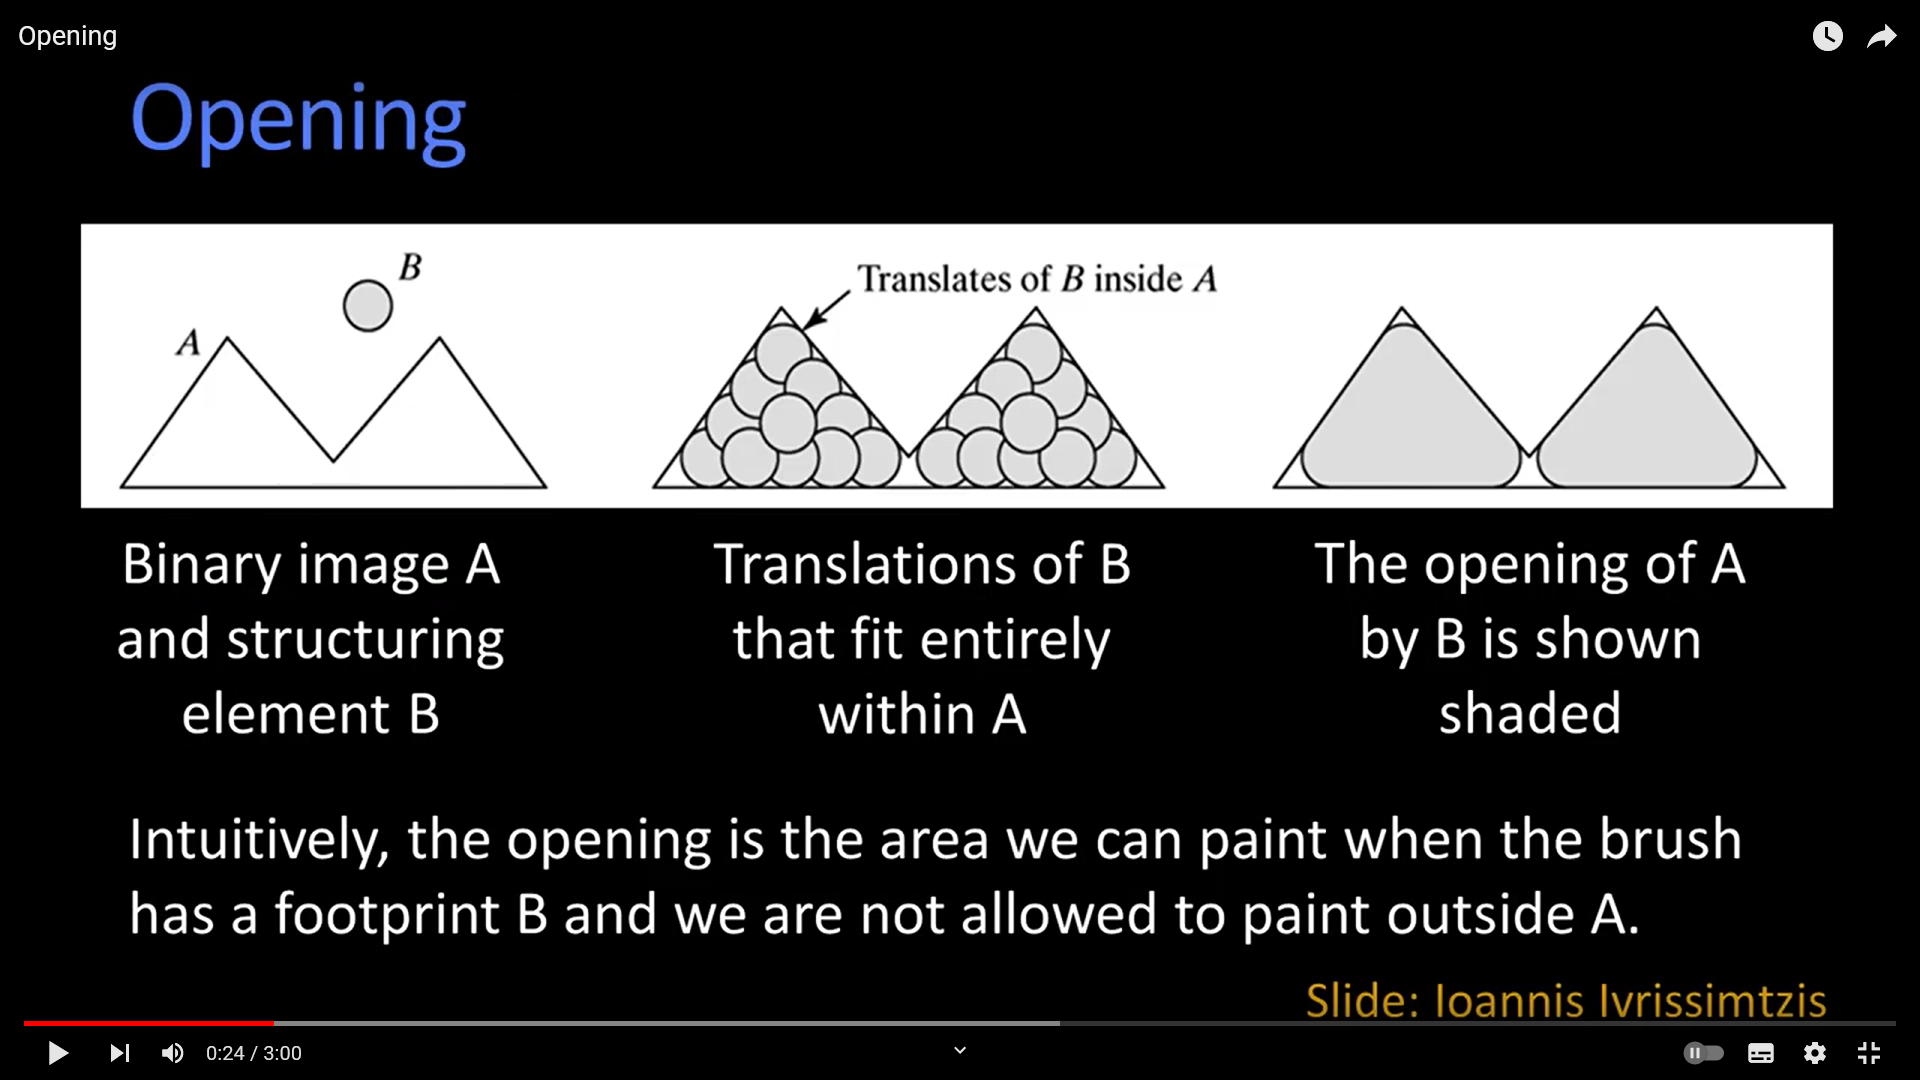
\includegraphics[width=0.8\textwidth]{figures/detection/opening.png}
    \caption{The opening of A by B.}
    \label{fig:opening}
\end{figure}

The holes and erroneously disjointed sections are removed using the morphological closing operation. The closing of A by B is the complement of the union of all translations of B that do not overlap A. This can be intuitively understood as illuminated in \autoref{fig:closing}.

\begin{figure}[h]
    \centering
    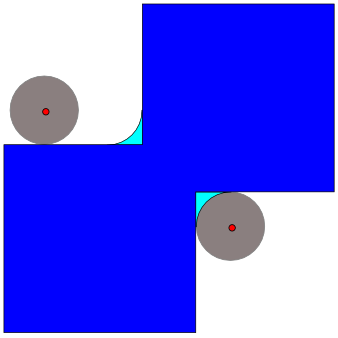
\includegraphics[width=0.8\textwidth]{figures/detection/closing.png}
    \caption{The closing of A by B.}
    \label{fig:closing}
\end{figure}

The structuring element B will be tuned to obtain the best results.

\paragraph{Connected components labelling}\mbox{}\\
The connected components labelling algorithm labels the connected components in a binary image. The algorithm works by iterating over the pixels in the image and assigning a label to each pixel. The label of a pixel is determined by the labels of the pixels in its neighbourhood. The neighbourhood of a pixel can be defined using either four or eight connectivity. 4 connectivity defines the neighbourhood of a pixel as the pixels to the left, right, top, and bottom of the pixel. 8 connectivity defines the neighbourhood of a pixel as the pixels to the left, right, top, bottom, top left, top right, bottom left, and bottom right of the pixel. The \gls{ccl} connectivity is shown in \autoref{fig:ccl_connectivity}.
% The algorithm is illustrated in \autoref{fig:connected_components_labelling}.

\begin{figure}[h]
    \centering
    \subfigure[Four connectivity.
        \label{fig:four_connectivity}]
    {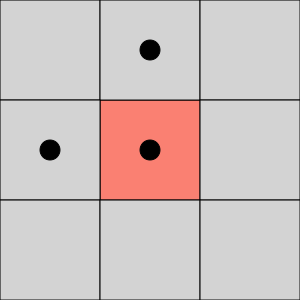
\includegraphics[width=0.2\textwidth]{figures/detection/square_4_connectivity.png}}
    \mbox{\hspace{1cm}}
    \subfigure[Eight connectivity.
        \label{fig:eight_connectivity}]
    {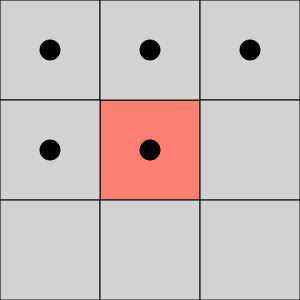
\includegraphics[width=0.2\textwidth]{figures/detection/square_8_connectivity.png}}
    \caption{Connected components labelling connectivity.}
    \label{fig:ccl_connectivity}
\end{figure}

\subsection{Software implementation and optimisation}
Only using red channel, \gls{gpu}, low resolution, etc.


\subsection{Final system integration and testing}
Real-time multi threading.

\newpage

%% End of File.

